\documentclass[tikz, border=10pt]{standalone}
\usepackage{tikz}
\usetikzlibrary{calc, positioning, shapes.geometric, backgrounds}

% Color definitions matching the nf-core metro map palette
\definecolor{linegray}{RGB}{140, 140, 140}
\definecolor{lineblue}{RGB}{20, 100, 245}
\definecolor{lineyellow}{RGB}{220, 175, 40}
\definecolor{linered}{RGB}{180, 20, 40}
\definecolor{linecyan}{RGB}{40, 180, 230}
\definecolor{linegreen}{RGB}{150, 185, 30}
\definecolor{linepurple}{RGB}{200, 160, 215}
\definecolor{lineblack}{RGB}{20, 20, 20}

\begin{document}

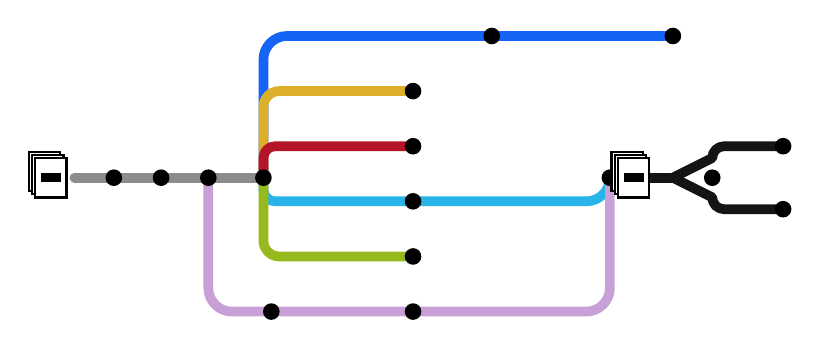
\begin{tikzpicture}[
    line/.style={draw, line width=3.5pt, line cap=round, line join=round},
    station/.style={circle, fill=black, inner sep=0pt, minimum size=6pt},
    icon/.style={rectangle, draw=black, fill=white, thick, minimum width=0.4cm, minimum height=0.5cm, inner sep=0pt}
]

% --- COORDINATE DEFINITIONS ---
% Main backbone entry
\coordinate (start) at (0, 0);
\coordinate (s1) at (0.5, 0);
\coordinate (s2) at (1.1, 0);
\coordinate (split_purple) at (1.7, 0);
\coordinate (split_main) at (2.4, 0);

% Branch end/station X-coordinates
\def\xmid{4.3}
\def\xmerge{6.8}
\def\xend{7.6}

% Y-coordinates for parallel tracks
\def\yblue{1.8}
\def\yyellow{1.1}
\def\yred{0.4}
\def\ycyan{-0.3}
\def\ygreen{-1.0}
\def\ypurple{-1.7}

% --- DRAW METRO LINES ---

% 1. Input Backbone (Gray)
\draw[line, linegray] (start) -- (split_main);

% 2. Top Blue Line (e.g., FastQC / Preprocessing)
\draw[line, lineblue] (split_main) -- (2.4, \yblue - 0.3) 
    arc [start angle=180, end angle=90, radius=0.3] -- (7.6, \yblue);

% 3. Yellow Line
\draw[line, lineyellow] (split_main) -- (2.4, \yyellow - 0.2) 
    arc [start angle=180, end angle=90, radius=0.2] -- (\xmid, \yyellow);

% 4. Dark Red Line
\draw[line, linered] (split_main) -- (2.4, \yred - 0.15) 
    arc [start angle=180, end angle=90, radius=0.15] -- (\xmid, \yred);

% 5. Cyan Line (Merging track)
\draw[line, linecyan] (split_main) -- (2.4, \ycyan + 0.15) 
    arc [start angle=180, end angle=270, radius=0.15] -- (6.5, \ycyan)
    arc [start angle=270, end angle=360, radius=0.3] -- (\xmerge, 0);

% 6. Green Line
\draw[line, linegreen] (split_main) -- (2.4, \ygreen + 0.2) 
    arc [start angle=180, end angle=270, radius=0.2] -- (\xmid, \ygreen);

% 7. Purple Line (Early split, bottom loop)
\draw[line, linepurple] (split_purple) -- (1.7, \ypurple + 0.3) 
    arc [start angle=180, end angle=270, radius=0.3] -- (6.5, \ypurple)
    arc [start angle=270, end angle=360, radius=0.3] -- (\xmerge, 0);

% 8. Output Black Fork
\draw[line, lineblack] (\xmerge, 0) -- (\xend, 0);
\draw[line, lineblack] (\xend, 0) -- (8.1, 0.25) arc [start angle=180, end angle=90, radius=0.15] -- (9.0, 0.4);
\draw[line, lineblack] (\xend, 0) -- (8.1, -0.25) arc [start angle=180, end angle=270, radius=0.15] -- (9.0, -0.4);


% --- STATIONS (BLACK DOTS) ---
% Backbone stations
\node[station] at (s1) {};
\node[station] at (s2) {};
\node[station] at (split_purple) {};
\node[station] at (split_main) {};

% Blue Line stations
\node[station] at (5.3, \yblue) {};
\node[station] at (7.6, \yblue) {};

% Middle caller terminals (\xmid)
\node[station] at (\xmid, \yyellow) {};
\node[station] at (\xmid, \yred) {};
\node[station] at (\xmid, \ycyan) {};
\node[station] at (\xmid, \ygreen) {};

% Purple Line stations
\node[station] at (2.5, \ypurple) {};
\node[station] at (\xmid, \ypurple) {};

% Merge & Output stations
\node[station] at (\xmerge, 0) {};
\node[station] at (8.1, 0) {};
\node[station] at (9.0, 0.4) {};
\node[station] at (9.0, -0.4) {};


% --- ICONS (Stacked Document Graphics) ---
% Input Data Icon (Left)
\begin{scope}[shift={(-0.3,0)}]
    \node[icon] at (-0.08, 0.08) {};
    \node[icon] at (-0.04, 0.04) {};
    \node[icon] at (0, 0) {};
    \draw[black, fill=black] (-0.12, -0.05) rectangle (0.12, 0.05);
\end{scope}

% Summary/Report Icon (Right before fork)
\begin{scope}[shift={(7.1,0)}]
    \node[icon] at (-0.08, 0.08) {};
    \node[icon] at (-0.04, 0.04) {};
    \node[icon] at (0, 0) {};
    \draw[black, fill=black] (-0.12, -0.05) rectangle (0.12, 0.05);
\end{scope}

\end{tikzpicture}

\end{document}